\section{Die Methode der kleinsten Quadrate}

In Anwendungssituationen wird man kaum erreichen, dass Modell und Messdaten exakt zusammenpassen. Ein Modell, das die Daten exakt interpoliert, wird in den seltensten Fällen ein brauchbares Modell sein.

Betrachten Sie dazu das folgende Beispiel. Ein Autofahrer hat mehrmals die mit seinem Auto getankte Benzinmenge und die gefahrenen Kilometer notiert:

\begin{center}
\begin{tabular}{|c|c|c|c|c|c|c|c|c|c|}
\hline
% \textbf{} & \textbf{1} & \textbf{2} & \textbf{3} & \textbf{4} & \textbf{5} & \textbf{6} & \textbf{7} & \textbf{8} & \textbf{9} \\
% \hline
\textbf{Strecke [km]} & 202 & 480 & 361 & 220 & 249 & 348 & 512 & 187 & 471 \\
\hline
\textbf{Benzin [l]} & 22.9 & 45.9 & 31.5 & 23.9 & 26.0 & 33.9 & 44.9 & 17.9 & 43.5 \\
\hline
\end{tabular}
\end{center}

\begin{center}
    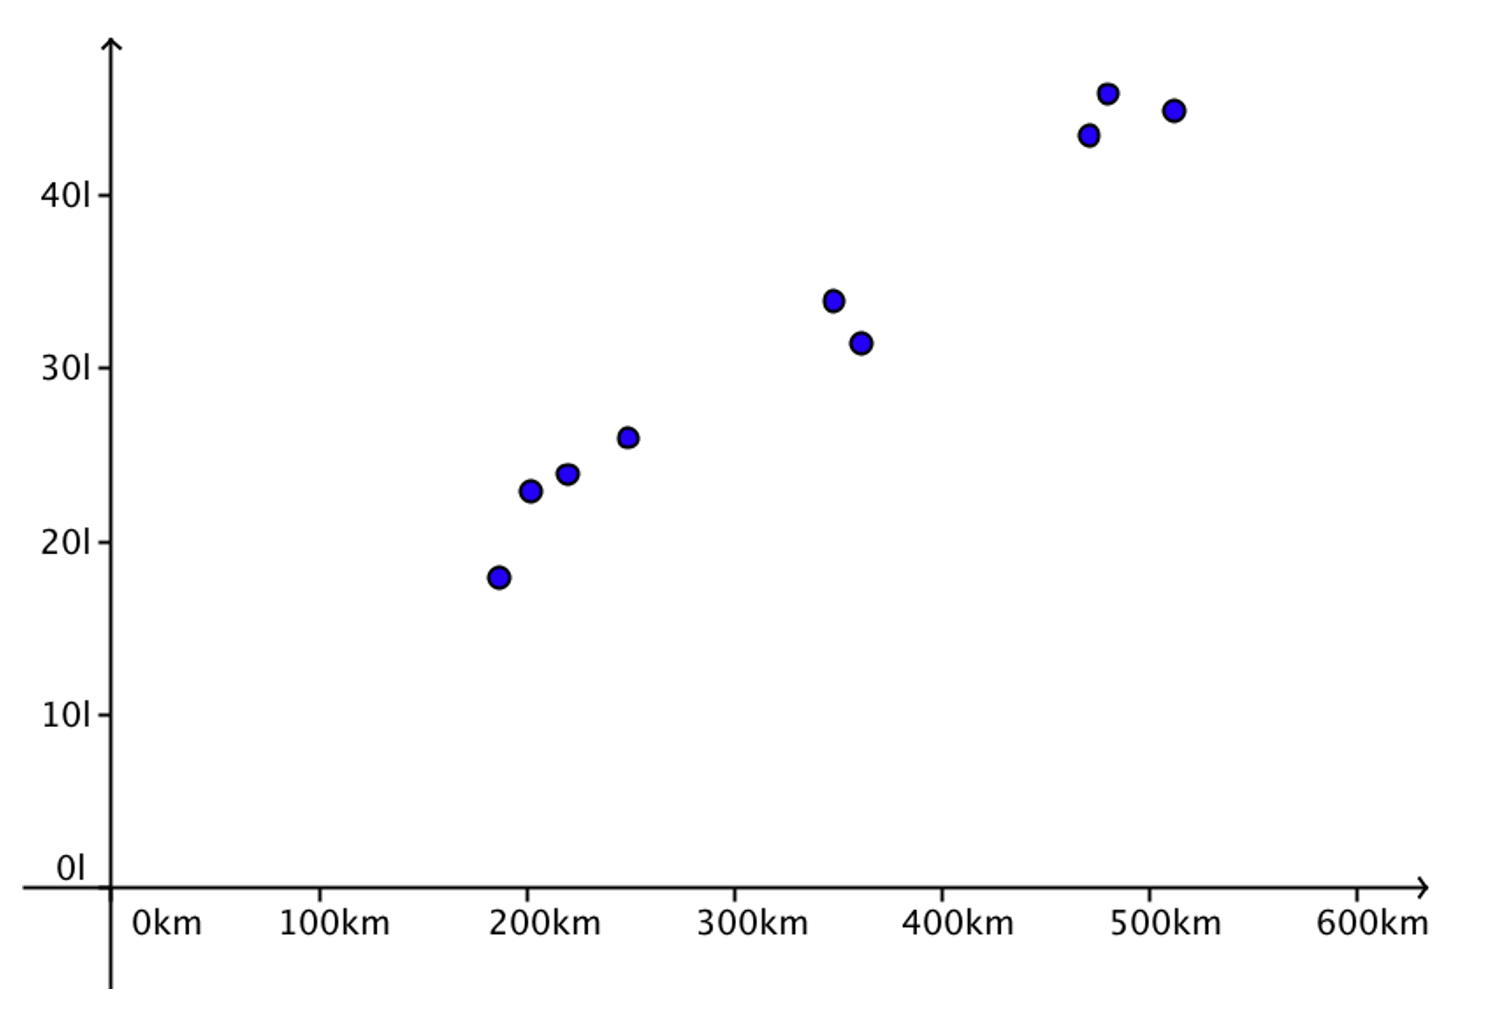
\includegraphics[width=0.5\textwidth]{media/introkleinsteQuadrate1.png}
\end{center}

Die 9 Messpunkte können durch eine Polynomfunktion 8. Grades exakt interpoliert werden. Die entsprechende Kurve sieht dann wie folgt aus:

\begin{center}
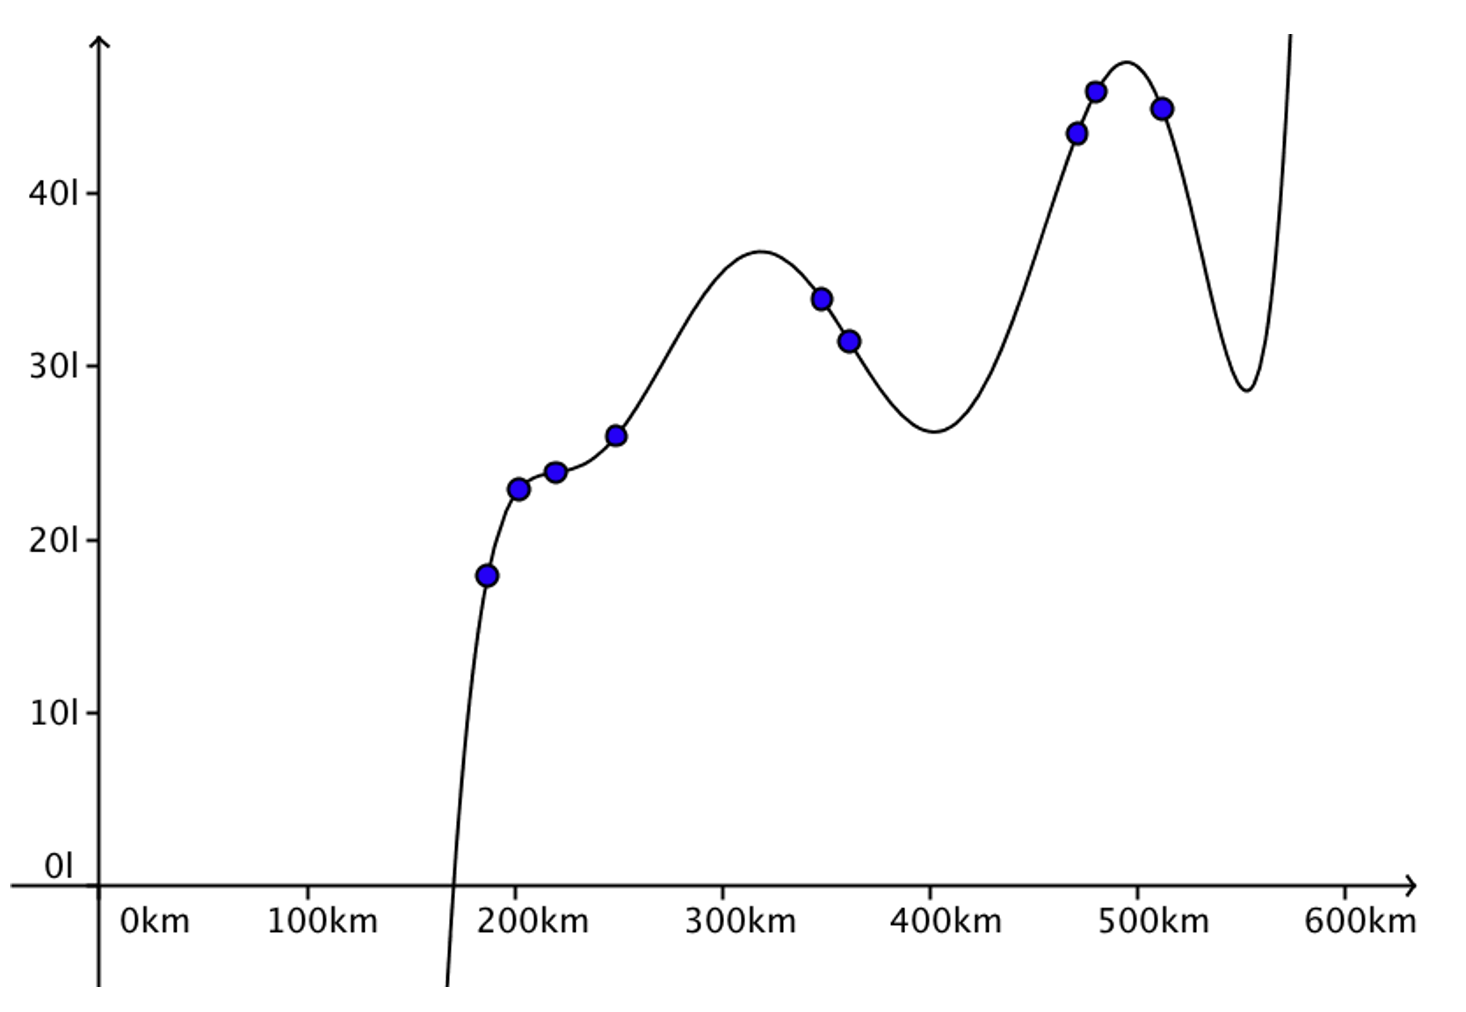
\includegraphics[width=0.5\textwidth]{media/introkleinstequadrate2.png}
\end{center}

Auch wenn das Polynom eine exakte Anpassung an die Messwerte leistet, so liefert es ein absurdes Modell. In diesem Fall ist es sinnvoll, von einem linearen Zusammenhang oder gar einer Proportionalität auszugehen. Damit lassen sich weitaus bessere Vorhersagen treffen. Das folgende Bild zeigt eine lineare Funktion, die sich den Messdaten annähert:

\begin{center}
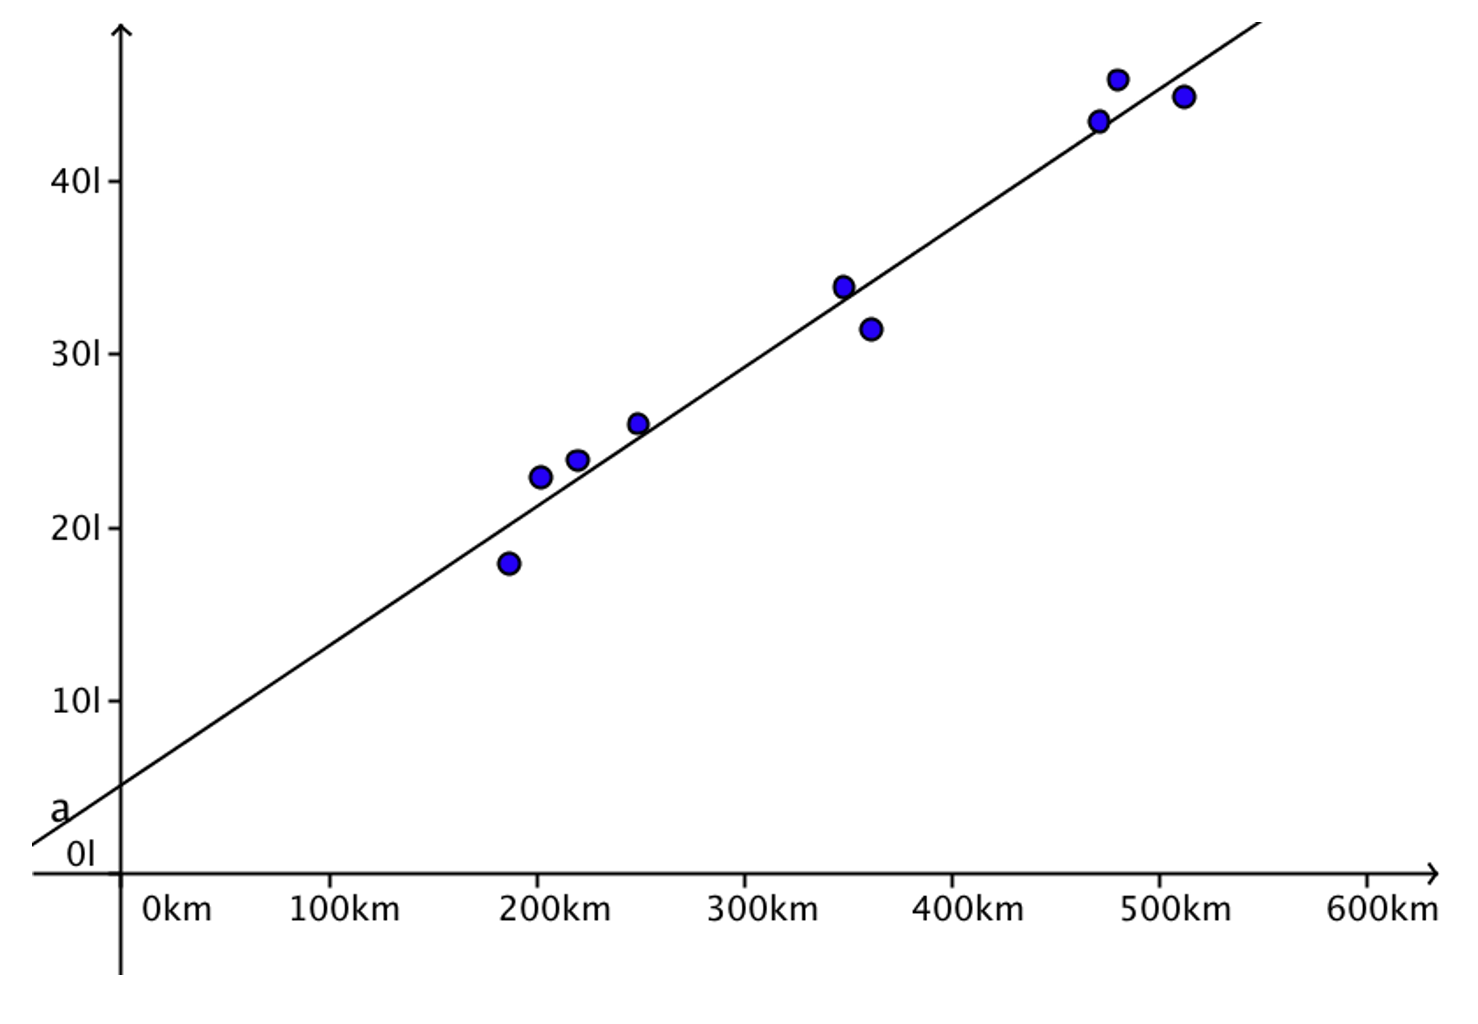
\includegraphics[width=0.5\textwidth]{media/introkleinstequadrate3.png}
\end{center}

Die Gerade in der Abbildung nennt man Regressionsgerade oder Ausgleichsgerade. Vielleicht haben Sie die Formel dafür bereits einmal angetroffen:

\begin{satz}
{Regressionsgerade}{}
Seien \( n \) Punkte \( P_1 (x_1, y_1), P_2 (x_2, y_2), \dots, P_n (x_n, y_n) \) gegeben.  
Die Gerade, welche sich im Sinne der kleinsten Quadrate den Punkten am besten nähert, ist \( g: y = mx + q \), mit  
\[
m = \frac{\sum_{k=1}^n (y_k - \overline{y}) x_k}{\sum_{k=1}^n (x_k - \overline{x}) x_k}, \quad q = \overline{y} - m \overline{x},
\]
wobei  
\[
\overline{x} = \frac{1}{n} \sum_{k=1}^n x_k, \quad \overline{y} = \frac{1}{n} \sum_{k=1}^n y_k
\]
die Mittelwerte der \( x \)- und \( y \)-Koordinaten der gegebenen Punkte sind.  
Die Gerade \( g \) nennt man \textbf{Regressions- oder Ausgleichsgerade}.
\end{satz}


In diesem Kapitel werden wir die Formel für die Regressionsgerade herleiten. Dabei werden wir unser Wissen über Extrema von Funktionen in zwei Variablen anwenden. Ausserdem werden wir ein allgemeines Prinzip kennenlernen, das viel weitreichender ist, als die Formel für die Ausgleichsgerade – die \textbf{Methode der kleinsten Quadrate}.

Diese Formel für die Regressionsgerade müssen Sie nicht lernen, die Methode der kleinsten Quadrate aber schon!

Um dieses Prinzip zu verstehen, werden wir so tun, als würden wir die Formel für die Regressionsgerade nicht kennen und in einem Beispiel mit wenigen Messpunkten eine passende lineare Funktion suchen.















\clearpage
\begin{LA}
{Methode der kleinsten Quadrate}{kleinsteQuadrate}
\textbf{Gegeben}: Messpunkte \( A(0,0), B(1,1), C(2,1), D(3,2) \)  

\textbf{Gesucht}: Eine lineare Funktion \( f(x) = mx + q \), die sich den Punkten annähert.

\begin{center}
    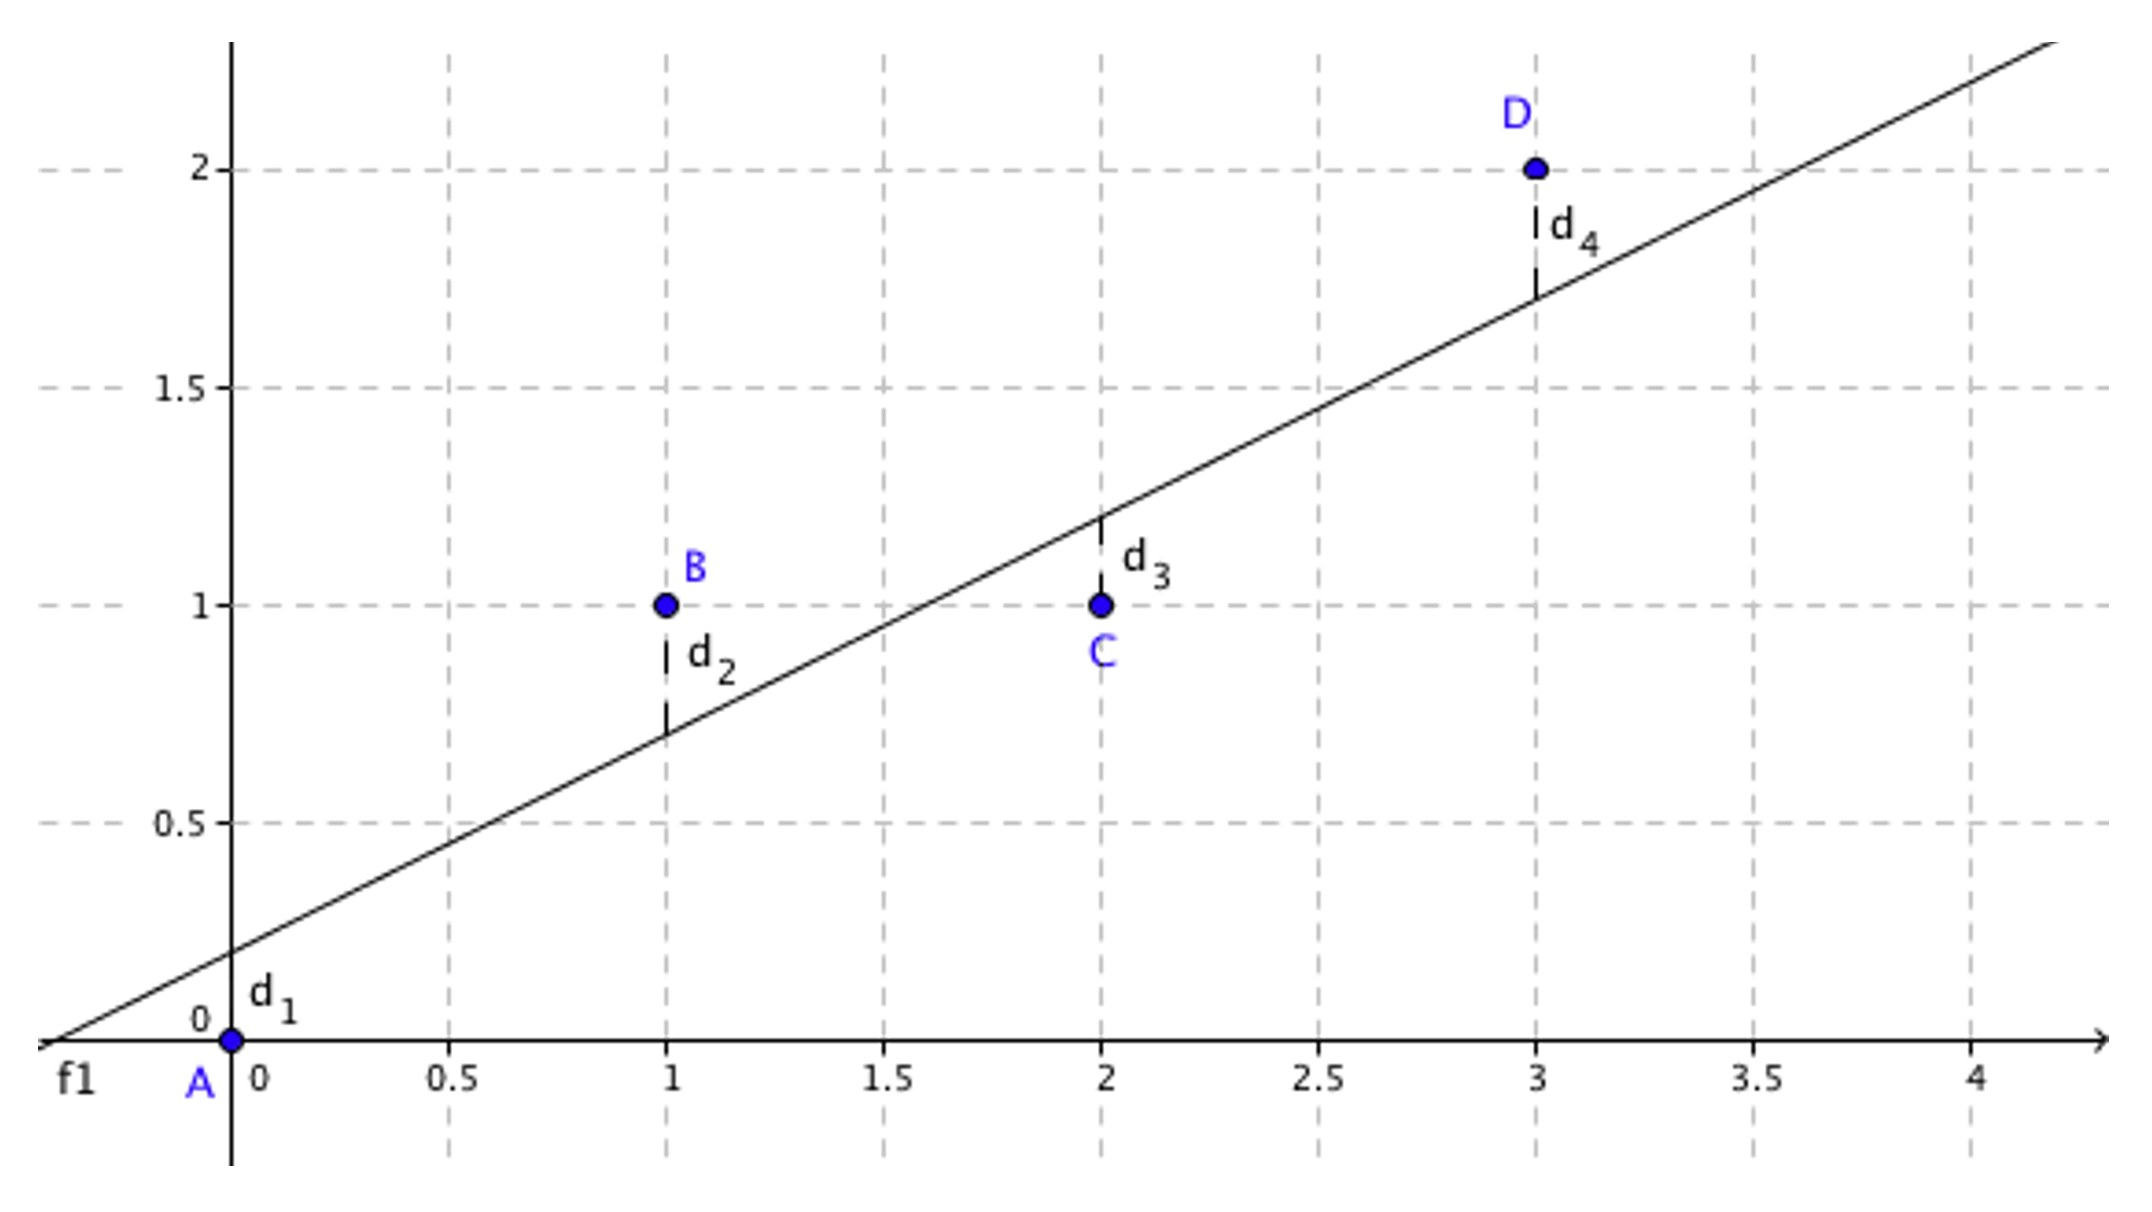
\includegraphics[width = 0.5 \textwidth]{media/kleinsteQuadrateLA.png}
\end{center}


\begin{enumerate}
    \item Betrachten Sie die Funktion \( f_1(x) = 0.5x + 0.2 \). Der Funktionswert an der Stelle \( x = 0 \) ist \( f_1(0) = 0.2 \). Der Messwert an der Stelle \( x = 0 \) ist 0 (siehe Punkt \( A \)). Die Abweichung beträgt also  
    \[
    d_1 = f_1(0) - 0 = 0.2 - 0 = 0.2
    \]
    Berechnen Sie analog die Abweichungen „Funktionswert minus Messwert“ \( d_2, d_3 \) und \( d_4 \) an den Stellen \( x = 1, x = 2 \) und \( x = 3 \). Wie gross ist die Summe der Abweichungen?  
    
    (Kontrolle: Summe \( = -0.2 \))
\end{enumerate}
\vspace*{4cm}



Wenn Sie stur nach der Formel „Funktionswert minus Messwert“ gerechnet haben, sind die Abweichungen \( d_1 \) und \( d_3 \) positiv, während \( d_2 \) und \( d_4 \) negativ sind. Das hat zur Folge, dass sich die Fehler in der Summe der Abweichungen zum Teil aufheben. Um das zu vermeiden, berechnet man die Summe der \textbf{Quadrate} der Abweichungen.  

\begin{enumerate}[resume]
    \item Berechnen Sie die Summe der Quadrate der Abweichungen  
    \[
    E = d_1^2 + d_2^2 + d_3^2 + d_4^2
    \]
    für die Funktion \( f_1(x) = 0.5x + 0.2 \).  
    \vspace*{2cm}
    %(Kontrolle: \( E = 0.26 \))


    \item Berechnen Sie die Summe der Quadrate der Abweichungen für die Funktionen \( f_2(x) = \frac{2}{3}x \) und \( f_3(x) = 1 \). Welche der Funktionen \( f_1, f_2 \) oder \( f_3 \) nähert sich den Punkten demnach am besten?  

    %(Kontrolle: \( E_2 = 0.\overline{2}, E_3 = 2 \))
\end{enumerate}


\vspace*{3cm}
Gibt es lineare Funktionen, welche für die vier vorgegebenen Punkte noch kleinere Summen von Abweichungsquadraten liefern als die vorgeschlagenen? Um diese Frage zu beantworten, betrachten wir eine allgemeine lineare Funktion \( f(x) = mx + q \).  

\begin{enumerate}[resume]
    \item Berechnen Sie für die vier vorgegebenen Punkte die Summe der Abweichungsquadrate \( E(m, q) \) in Abhängigkeit der Parameter \( m \) und \( q \).  
    
    (Kontrolle: \( E(m, q) = q^2 + (m + q - 1)^2 + (2m + q - 1)^2 + (3m + q - 2)^2 \))
    
\end{enumerate}
\vspace*{5cm}
%\clearpage
Wir wollen nun die Werte \( m \) und \( q \) bestimmen, für welche die Summe der Quadrate der Abweichungen \( E \) minimal wird.  


\begin{enumerate}[resume]
    \item An welcher Stelle \( (m, q) \) ist die Funktion \( E(m, q) \) minimal?  
    
    (Kontrolle: \( m = \frac{3}{5}, q = \frac{1}{10} \))
    %\vspace*{10cm}
\end{enumerate}
\end{LA}

\clearpage


\begin{definition}
{Methode der kleinsten Quadrate}{}
Seien \( n \) (Mess-)Punkte \( P_1 (x_1, y_1), P_2 (x_2, y_2), \dots, P_n (x_n, y_n) \) gegeben.

Sei $y=f(x)$ eine Funktion mit $k$ frei wählbare Parameter $a_1, a_2, \dots, a_k$.

Wir sagen, dass die Funktion $f(x)$ den Zusammenhang zwischen den Daten im Sinne der kleinsten Quadrate möglichst gut beschreibt, wenn die Parameter so gewählt sind, dass die Summe der quadrierten Abweichungen 

$$E(a_1, a_2 \dots, a_n) = \sum_{i=1}^n (f(x_i)- y_i)^2 $$

minimal ist.

\end{definition}

Bemerkungen:
\begin{itemize}
    \item Wenn man die Überlegung von \cref*{LA:kleinsteQuadrate} allgemein mit $n$ Messpunkten durchführt, erhält man die bekannte Formel für die Regressionsgerade.
    \item Vielleicht haben Sie es bemerkt: Wir haben die Methode der kleinsten Quadrate bereits einmal verwendet, um den Fehler im neuronalen Netzwerk zu minimieren.
\end{itemize}

\begin{ueb}
{}{}
\begin{enumerate}
    % \item Betrachten Sie die Messdaten:
    % \[
    % \begin{array}{|c|c|c|c|c|c|c|c|c|}
    % \hline
    % x & 1 & 3 & 4 & 6 & 8 & 9 & 11 & 14 \\
    % \hline
    % y & 1 & 2 & 4 & 4 & 5 & 7 & 8 & 9 \\
    % \hline
    % \end{array}
    % \]

    % \begin{enumerate}
    %     \item Bestimmen Sie die Regressionsgerade.

    %     \item Bestimmen Sie die Regressionsgerade, nachdem Sie die Rolle von \( x \) und \( y \) vertauscht haben.
    
    %     \item Zeichnen Sie die Punkte mit Excel in einem «xy-Diagramm». Unter den Diagrammoptionen können Sie eine Trendlinie hinzufügen und in den Einstellungen wählen, dass deren Gleichung angezeigt wird. Vergleichen Sie Ihr Resultat mit der Excel-„Trendlinie“.
    % \end{enumerate}
    
    
    \item Gegeben sind die vier Punkte \( A(-1 , 0), B(0 , 1), C(1 , 1), D(2 , -1) \).  
    Bestimmen Sie die Funktion
    $$f(x) = ax^2+bx+c ,$$
    die sich im Sinne der kleinsten Quadrate den Punkten am besten nähert.

    \item Gegeben \( n \) Punkte \( P_1 (x_1 , y_1), P_2 (x_2 , y_2), \dots, P_n (x_n , y_n) \).  \\ 
    Gesucht ist ein Kreis \( K: x^2 + y^2 = r^2 \) um den Ursprung mit Radius \( r \), der sich den Punkten nähert. Dabei soll der Radius \( r \) so gewählt werden, dass  
    \[
    E(r) = \sum_{k=1}^n \left( x_k^2 + y_k^2 - r^2 \right)^2
    \]
    minimal ist. Geben Sie eine Formel für \( r \) an. \footnote{Auf eine ähnliche Art konnte Gauss im Jahr 1801 die Bahn des Zwergplaneten Ceres berechnen. Weil seine Voraussagen viel präziser als jene der führenden Astronomen war, hat der 24 jährige Gauss damit einiges Aufsehen erregt!}
\end{enumerate}
    
\end{ueb}

\clearpage
\emph{Lösungen}
\begin{enumerate}
    % \item \textbf{Regressionsgerade:}
    % \begin{enumerate}
    %     \item \( y = \frac{7}{11}x + \frac{6}{11} \)
    %     \item \( y = \frac{3}{2}x - \frac{1}{2} \) (Weil die Abweichungen in senkrechter Richtung gemessen werden, spielt es eine Rolle, welche Werte als In- und welche als Output interpretiert werden.)
    %     \item Die Trendlinie entspricht genau der Regressionsgerade.
    % \end{enumerate}

    \item \textbf{Ansatz:} \( y = ax^2 + bx + c \). Die Gleichung \( \vec \nabla E(a, b, c) = 0 \) ist ein \( 3 \times 3 \)-System mit genau einer Lösung. Diese muss ein Minimum sein. Die gesuchte Parabel hat die Gleichung:
    \[
    y = -\frac{3}{4}x^2 + \frac{9}{20}x + \frac{23}{20}
    \]

    \item \( R = \pm \sqrt{\frac{\sum (x_k^2 + y_k^2)}{n}} \), wobei die negative Lösung als Radius wegfällt.
\end{enumerate}